%%% Copyright (C) 2018 Vincent Goulet
%%%
%%% Ce fichier fait partie du projet «Méthodes numériques en actuariat»
%%% http://github.com/vigou3/methodes-numeriques-en-actuariat
%%%
%%% Cette création est mise à disposition selon le contrat
%%% Attribution-Partage dans les mêmes conditions 4.0
%%% International de Creative Commons.
%%% http://creativecommons.org/licenses/by-sa/4.0/

%%% Copyright (C) 2018 Vincent Goulet
%%%
%%% Ce fichier fait partie du projet
%%% «Méthodes numériques en actuariat avec R»
%%% http://github.com/vigou3/methodes-numeriques-en-actuariat
%%%
%%% Cette création est mise à disposition selon le contrat
%%% Attribution-Partage dans les mêmes conditions 4.0
%%% International de Creative Commons.
%%% http://creativecommons.org/licenses/by-sa/4.0/

\documentclass[letterpaper,11pt,x11names,english,french]{memoir}
  \usepackage{natbib,url}
  \usepackage{babel}
  \usepackage[autolanguage]{numprint}
  \usepackage{amsmath,amsthm}
  \usepackage[noae]{Sweave}
  \usepackage{graphicx}
  \usepackage{actuarialangle}          % \angl et al.
  \usepackage{framed}                  % env. snugshade*, oframed
  \usepackage{paralist}
  \usepackage[shortlabels]{enumitem}   % configuration listes
  \usepackage[absolute]{textpos}       % éléments des pages de titre
  \usepackage{relsize}                 % \smaller et al.
  \usepackage{manfnt}                  % \mantriangleright (puce)
  \usepackage{metalogo}                % \XeLaTeX logo
  \usepackage{fontawesome}             % icônes \fa*
  \usepackage{awesomebox}              % boites info, important, etc.
  \usepackage{answers}                 % exercices et solutions
  \usepackage{listings}                % code informatique
  \usepackage{xr}                      % références entre parties

  %%% =======================================================
  %%%  Informations de publication (sauf titre de la partie)
  %%% =======================================================
  \title{Méthodes numériques en actuariat avec R}
  \author{Vincent Goulet}
  \renewcommand{\year}{2018}
  \renewcommand{\month}{01}
  \newcommand{\ghurl}{https://github.com/vigou3/methodes-numeriques-en-actuariat/}

  %%% ===================
  %%%  Style du document
  %%% ===================

  %% Polices de caractères
  \usepackage{fontspec}
  \usepackage[bold-style=upright]{unicode-math}
  \defaultfontfeatures{Scale=0.92}
  \setmainfont[Ligatures=TeX,Numbers=OldStyle]{Lucida Bright OT}
  \setmathfont{Lucida Bright Math OT}
  \setmonofont{Lucida Grande Mono DK}
  \setsansfont[Scale=1.0,Numbers=OldStyle]{Myriad Pro}
  \newfontfamily\fullcaps[Letters=Uppercase,Numbers=Uppercase]{Myriad Pro}
  \usepackage[babel=true]{microtype}
  \usepackage{icomma}

  %% Couleurs
  \usepackage{xcolor}
  \definecolor{comments}{rgb}{0.7,0,0}           % commentaires
  \definecolor{link}{rgb}{0,0.4,0.6}             % liens internes
  \definecolor{url}{rgb}{0.6,0,0}                % liens externes
  \definecolor{citation}{rgb}{0,0.5,0}           % citations
  \definecolor{codebg}{named}{LightYellow1}      % fond code R
  \definecolor{prob}{named}{orange}              % encadrés «problème»
  \definecolor{rouge}{rgb}{0.85,0,0.07} % rouge bandeau identitaire
  \definecolor{or}{rgb}{1,0.8,0}        % or bandeau identitaire

  %% Hyperliens
  \usepackage{hyperref}
  \hypersetup{%
    pdfauthor = {Vincent Goulet},
    colorlinks = {true},
    linktocpage = {true},
    urlcolor = {url},
    linkcolor = {link},
    citecolor = {citation},
    pdfpagemode = {UseOutlines},
    pdfstartview = {Fit},
    bookmarksopen = {true},
    bookmarksnumbered = {true},
    bookmarksdepth = {subsubsection}}
  \setlength{\XeTeXLinkMargin}{1pt}

  %% Étiquettes de \autoref (redéfinitions compatibles avec babel).
  %% Attention! Les % à la fin des lignes sont importants sinon des
  %% blancs apparaissent dès que la commande \selectlanguage est
  %% utilisée... comme dans la bibliographie, par exemple.
  \addto\extrasfrench{%
    \def\algorithmeautorefname{algorithme}%
    \def\appendixautorefname{annexe}%
    \def\definitionautorefname{définition}%
    \def\figureautorefname{figure}%
    \def\exempleautorefname{exemple}%
    \def\exerciceautorefname{exercice}%
    \def\subfigureautorefname{figure}%
    \def\subsectionautorefname{section}%
    \def\subtableautorefname{tableau}%
    \def\tableautorefname{tableau}%
    \def\thmautorefname{théorème}%
  }

  %% Table des matières (inspirée de classicthesis.sty)
  \renewcommand{\cftchapterleader}{\hspace{1.5em}}
  \renewcommand{\cftchapterafterpnum}{\cftparfillskip}
  \renewcommand{\cftsectionleader}{\hspace{1.5em}}
  \renewcommand{\cftsectionafterpnum}{\cftparfillskip}

  %% Titres des chapitres
  \chapterstyle{hangnum}
  \renewcommand{\chaptitlefont}{\normalfont\Huge\sffamily\bfseries\raggedright}

  %% Marges, entêtes et pieds de page
  \setlength{\marginparsep}{7mm}
  \setlength{\marginparwidth}{13mm}
  \setlength{\headwidth}{\textwidth}
  \addtolength{\headwidth}{\marginparsep}
  \addtolength{\headwidth}{\marginparwidth}

  %% Titres des sections et sous-sections
  \setsecheadstyle{\normalfont\Large\sffamily\bfseries\raggedright}
  \setsubsecheadstyle{\normalfont\large\sffamily\bfseries\raggedright}
  \maxsecnumdepth{subsection}
  \setsecnumdepth{subsection}

  %% Listes. Paramétrage avec enumitem.
  \setlist[enumerate]{leftmargin=*,align=left}
  \setlist[enumerate,2]{label=\alph*),labelsep=*,leftmargin=1.5em}
  \setlist[enumerate,3]{label=\roman*),labelsep=*,leftmargin=1.5em,align=right}
  \setlist[itemize]{leftmargin=*,align=left}

  %% Options de babel
  \frenchbsetup{StandardItemizeEnv=true,%
    ThinSpaceInFrenchNumbers=true,
    ItemLabeli=\mantriangleright,
    ItemLabelii=\textendash,
    og=«, fg=»}
  \addto\captionsfrench{\def\figurename{{\scshape Fig.}}}
  \addto\captionsfrench{\def\tablename{{\scshape Tab.}}}

  %% Sections de code source
  \lstloadlanguages{R}
  \lstset{language=R,
    basicstyle=\small\ttfamily\NoAutoSpacing,
    keywordstyle=\mdseries,
    commentstyle=\color{comments}\slshape,
    extendedchars=true,
    showstringspaces=false}

  %%% =========================
  %%%  Nouveaux environnements
  %%% =========================

  %% Environnements d'exemples et al.
  \theoremstyle{plain}
  \newtheorem{algorithme}{Algorithme}[chapter]
  \newtheorem{thm}{Théorème}[chapter]

  \theoremstyle{definition}
  \newtheorem{exemple}{Exemple}[chapter]
  \newtheorem{definition}{Définition}[chapter]
  \newtheorem*{astuce}{Astuce}

  \theoremstyle{remark}
  \newtheorem*{remarque}{Remarque}
  \newtheorem*{remarques}{Remarques}
  \newenvironment{rem}{\begin{remarque} \mbox{}}{\end{remarque}}
  \newenvironment{rems}{\begin{remarques} \mbox{}}{\end{remarques}}

  %% Redéfinition de l'environnement titled-frame de framed.sty avec
  %% deux modifications: épaisseur des filets réduite de 2pt à 1pt;
  %% "(suite)" plutôt que "(cont)" dans la barre de titre
  %% lorsque l'encadré se poursuit après un saut de page.
  \renewenvironment{titled-frame}[1]{%
    \def\FrameCommand{\fboxsep8pt\fboxrule1pt
      \TitleBarFrame{\textbf{#1}}}%
    \def\FirstFrameCommand{\fboxsep8pt\fboxrule1pt
      \TitleBarFrame[$\blacktriangleright$]{\textbf{#1}}}%
    \def\MidFrameCommand{\fboxsep8pt\fboxrule1pt
      \TitleBarFrame[$\blacktriangleright$]{\textbf{#1\ (suite)}}}%
    \def\LastFrameCommand{\fboxsep8pt\fboxrule1pt
      \TitleBarFrame{\textbf{#1\ (suite)}}}%
    \MakeFramed{\advance\hsize-16pt \FrameRestore}}%
  {\endMakeFramed}

  %% Encadré générique avec titre basé sur titled-frame, ci-dessus.
  %% Sert pour les listes d'objectifs et les encadrés reliés aux
  %% problèmes (mises en situation) dans les chapitres. Arguments:
  %% couleur du cadre (optionnel; noir par défaut) et titre de la
  %% boîte (obligatoire).
  \newenvironment{emphbox}[2][black]{%
    \colorlet{TFFrameColor}{#1}%
    \colorlet{TFTitleColor}{white}%
    \begin{titled-frame}{\sffamily #2}%
      \setlength{\parindent}{0pt}}%
    {\end{titled-frame}}

  %% Liste d'objectifs au début des chapitres
  \newenvironment{objectifs}{%
    \begin{emphbox}{\rule[-7pt]{0pt}{20pt} Objectifs du chapitre}
      \begin{itemize}[nosep]
        \small\sffamily}%
      {\end{itemize}\end{emphbox}}

  %% Problèmes (mises en situation) des chapitres: énoncé au début du
  %% chapitre; astuces en cours de chapitre; solution à la fin
  %% du chapitre.
  \newenvironment{prob-enonce}{%
    \begin{emphbox}[prob]{{\normalfont\faCogs}\; Énoncé du problème}}%
    {\end{emphbox}}
  \newenvironment{prob-astuce}{%
    \begin{emphbox}[prob]{{\normalfont\faBolt}\; Astuce}}%
    {\end{emphbox}}
  \newenvironment{prob-solution}{%
    \begin{emphbox}[prob]{{\normalfont\faLightbulbO}\; Solution du problème}}%
    {\end{emphbox}}

  %% Environnements de Sweave. Les environnements Sinput et Soutput
  %% utilisent Verbatim (de fancyvrb). On les réinitialise pour
  %% enlever la configuration par défaut de Sweave, puis on réduit
  %% l'écart entre les blocs Sinput et Soutput.
  \DefineVerbatimEnvironment{Sinput}{Verbatim}{}
  \DefineVerbatimEnvironment{Soutput}{Verbatim}{}
  \fvset{listparameters={\setlength{\topsep}{0pt}}}

  %% L'environnement Schunk est complètement redéfini en un hybride
  %% des environnements snugshade* et leftbar de framed.sty.
  \makeatletter
  \renewenvironment{Schunk}{%
    \setlength{\topsep}{1pt}
    \def\FrameCommand##1{\hskip\@totalleftmargin
       \vrule width 2pt\colorbox{codebg}{\hspace{3pt}##1}%
      % There is no \@totalrightmargin, so:
      \hskip-\linewidth \hskip-\@totalleftmargin \hskip\columnwidth}%
    \MakeFramed {\advance\hsize-\width
      \@totalleftmargin\z@ \linewidth\hsize
      \advance\labelsep\fboxsep
      \@setminipage}%
  }{\par\unskip\@minipagefalse\endMakeFramed}
  \makeatother

  %% Exercices et réponses
  \Newassociation{sol}{solution}{solutions}
  \Newassociation{rep}{reponse}{reponses}
  \newcounter{exercice}[chapter]
  \renewcommand{\theexercice}{\thechapter.\arabic{exercice}}
  \newenvironment{exercice}[1][]{%
    \begin{list}{}{%
        \refstepcounter{exercice}
        \ifthenelse{\equal{#1}{nosol}}{%
          \renewcommand{\makelabel}{\bfseries\theexercice}}{%
          \hypertarget{ex:\theexercice}{}
          \Writetofile{solutions}{\protect\hypertarget{sol:\theexercice}{}}
          \renewcommand{\makelabel}{%
            \bfseries\protect\hyperlink{sol:\theexercice}{\theexercice}}}
        \settowidth{\labelwidth}{\bfseries\theexercice}
        \setlength{\leftmargin}{\labelwidth}
        \addtolength{\leftmargin}{\labelsep}
        \setlist[enumerate,1]{label=\alph*),labelsep=*,leftmargin=1.5em}
        \setlist[enumerate,2]{label=\roman*),labelsep=0.5em,align=right}}
      \item}%
      {\end{list}}
  \renewenvironment{solution}[1]{%
    \begin{list}{}{%
        \renewcommand{\makelabel}{%
          \bfseries\protect\hyperlink{ex:#1}{#1}}
        \settowidth{\labelwidth}{\bfseries #1}
        \setlength{\leftmargin}{\labelwidth}
        \addtolength{\leftmargin}{\labelsep}
        \setlist[enumerate,1]{label=\alph*),labelsep=*,leftmargin=1.5em}
        \setlist[enumerate,2]{label=\roman*),labelsep=0.5em,align=right}}
    \item}%
    {\end{list}}
  \renewenvironment{reponse}[1]{%
    \begin{enumerate}[label=\textbf{#1}]
    \item}%
    {\end{enumerate}}

  %% Redéfinition de l'environnement de matrices de amsmath pour
  %% aligner les colonnes à droite. Pris dans
  %% <http://texblog.net/latex-archive/maths/matrix-align-left-right/>
  \makeatletter
  \renewcommand*\env@matrix[1][r]{\hskip -\arraycolsep
    \let\@ifnextchar\new@ifnextchar
    \array{*\c@MaxMatrixCols #1}}
  \makeatother

  %%% =====================
  %%%  Nouvelles commandes
  %%% =====================

  %% Noms de fonctions, code, etc.
  \newcommand{\code}[1]{\texttt{#1}}
  \newcommand{\pkg}[1]{\textbf{#1}}

  %% Hyperlien avec symbole de lien externe juste après; second
  %% argument peut être vide pour afficher l'url comme lien
  %% [https://tex.stackexchange.com/q/53068/24355 pour procédure de
  %% test du second paramètre vide]
  \newcommand{\link}[2]{%
    \def\param{#2}%
    \ifx\param\empty
      \href{#1}{\nolinkurl{#1}~\raisebox{-0.1ex}{\smaller\faExternalLink}}%
    \else
      \href{#1}{#2~\raisebox{-0.1ex}{\smaller\faExternalLink}}%
    \fi
  }

  %% Indications de capsule vidéo
  \newcommand{\capsule}[2]{\href{#1}{#2}\marginpar{%
      \href{#1}{\raisebox{-0.5em}[0em][0em]{\HUGE\faYoutubePlay}}}}

  %% Boites additionnelles (basées sur awesomebox.sty) pour remarques
  %% spécifiques à macOS et pour les changements au fil de la lecture.
  \newcommand{\osxbox}[1]{%
    \awesomebox{\faApple}{\aweboxrulewidth}{black}{#1}}
  \newcommand{\gotorbox}[1]{%
    \awesomebox{\faMapSigns}{\aweboxrulewidth}{black}{\sffamily #1}}

  %% Boite pour le nom du fichier de script correspondant au début des
  %% sections d'exemples.
  \newcommand{\scriptfile}[1]{%
    \begingroup
    \noindent
    \mbox{%
      \makebox[3mm][l]{\raisebox{-0.5pt}{\small\faChevronCircleDown}}\;%
      \smaller[1] {\sffamily Fichier d'accompagnement} {\ttfamily #1}}
    \endgroup}

  %% Lien vers GitHub dans la page de notices
  \newcommand{\viewsource}[1]{%
    \href{#1}{%
      Voir sur GitHub \raisebox{-1pt}{\footnotesize\faGithub}}}

  %% Raccourcis usuels vg
  \newcommand{\pt}{{\scriptscriptstyle \Sigma}}
  \newcommand{\abs}[1]{\lvert #1 \rvert}
  \newcommand{\norme}[1]{\lVert #1 \rVert}
  \newcommand{\mat}[1]{\symbf{#1}}
  \newcommand{\diag}{\operatorname{diag}}
  \newcommand{\Esp}[1]{E\! \left[ #1 \right]}
  \newcommand{\esp}[1]{E [ #1 ]}
  \newcommand{\Var}[1]{\operatorname{Var}\! \left[ #1 \right]}
  \newcommand{\var}[1]{\operatorname{Var} [ #1 ]}
  \newcommand{\Prob}[1]{\operatorname{Pr}\! \left[ #1 \right]}
  \newcommand{\prob}[1]{\operatorname{Pr} [ #1 ]}
  \newcommand{\R}{\symbb{R}}    % ensemble des réels

  %% Traitement du titre de partie
  \makeatletter
  \newcommand{\@parttitle}{}
  \newcommand{\parttitle}[1]{\renewcommand{\@parttitle}{#1}}
  \newcommand{\theparttitle}{\@parttitle}
  \makeatother

  %%% =======
  %%%  Varia
  %%% =======

  %% Sous-tableaux et figures
  \newsubfloat{table}
  \newsubfloat{figure}

  %% Style de la bibliographie
  \bibliographystyle{francais}

  %% Longueurs pour la composition des pages couvertures avant et
  %% arrière.
  \newlength{\banderougewidth} \newlength{\banderougeheight}
  \newlength{\bandeorwidth}    \newlength{\bandeorheight}
  \newlength{\imageheight}
  \newlength{\logoheight}
  \newlength{\gapwidth}

  %% Aide pour la césure
  \hyphenation{%
    con-gru-en-tiels
    con-naî-tre
    con-sole
    cons-tante
    con-tenu
    con-trôle
    hexa-dé-ci-mal
    nom-bre
    puis-que
  }

  \usepackage{multicol}         % environnement multicols

  %%% Titre de la partie et image de couverture
  \parttitle{Algèbre linéaire}
  \hypersetup{pdftitle = {\thetitle\ - \theparttitle}}
  \newcommand{\imagefile}{Furcifer-lateralis}

  %%% Numérotation des chapitres
  \setcounter{chapter}{6}

  %%% Commmandes algèbre linéaire
  \newcommand{\tr}{\mathrm{tr}}
  \newcommand{\pscal}[2]{\langle #1, #2 \rangle}

  %% Longueur utilisée dans les solutions
  \newlength{\ocolumnsep}

%  \includeonly{pagegarde,notices}

\begin{document}

\frontmatter

\pagestyle{empty}

%%% Copyright (C) 2018 Vincent Goulet
%%%
%%% Ce fichier fait partie du projet
%%% «Méthodes numériques en actuariat avec R»
%%% http://github.com/vigou3/methodes-numeriques-en-actuariat
%%%
%%% Cette création est mise à disposition selon le contrat
%%% Attribution-Partage dans les mêmes conditions 4.0
%%% International de Creative Commons.
%%% http://creativecommons.org/licenses/by-sa/4.0/

%%%
%%% Page de titre
%%%

\begingroup
\TPGrid{3}{36}
\textblockorigin{0mm}{0mm}
\setlength{\parindent}{0mm}
\setlength{\imageheight}{29\TPVertModule}
\setlength{\banderougewidth}{2\TPHorizModule}
\setlength{\banderougeheight}{\TPVertModule}
\setlength{\bandeorwidth}{\TPHorizModule}
\setlength{\bandeorheight}{\banderougeheight}
\setlength{\logoheight}{2.5\TPVertModule}
\setlength{\gapwidth}{1.5pt}
\addtolength{\bandeorwidth}{-\gapwidth}
\addtolength{\imageheight}{-\gapwidth}
\setlength{\fboxrule}{3pt}
\setlength{\fboxsep}{0pt}

\def\titlefmt{%
  \sffamily\bfseries\fontsize{42}{42}\selectfont\thetitle}
\def\parttitlefmt{%
  \sffamily\mdseries\fontsize{30}{30}\selectfont\theparttitle}
\def\authorfmt{%
  \sffamily\bfseries\fontsize{25}{25}\selectfont\theauthor}
\def\affiliation{%
  \sffamily\mdseries\fontsize{22}{22}\selectfont
  Professeur titulaire \\
  École d'actuariat, Université Laval \\[12mm]
  Avec la collaboration de \\
  \bfseries\fontsize{25}{30}\selectfont
  Laurent Caron}
\def\edition{%
  \sffamily\mdseries\fontsize{22}{22}\selectfont
  Édition {\fullcaps\year}.\month}

%% bandeau identitaire
\begin{textblock*}{\paperwidth}[0,1](0mm,30\TPVertModule)
  \textcolor{rouge}{\rule{\banderougewidth}{\banderougeheight}}% % bande rouge
  \rule{\gapwidth}{0pt}%                                         % filet
  \textcolor{or}{\rule{\bandeorwidth}{\bandeorheight}}           % bande or
\end{textblock*}

%% logo UL
\begin{textblock*}{\TPHorizModule}(2\TPHorizModule,31\TPVertModule)
  \rule{\gapwidth}{0pt}%                                         % filet
  
\includegraphics[height=\logoheight,%
                   keepaspectratio=true]{../share/ul_p}
\end{textblock*}

%% image de fond
\begin{textblock*}{\paperwidth}(0mm,0mm)
  \includegraphics[width=\paperwidth,%
                   keepaspectratio=true]{\imagefile}
\end{textblock*}

%% titre
\begin{textblock*}{2.3\TPHorizModule}(0.35\TPHorizModule,4\TPVertModule)
  \textcolor{white}{\titlefmt}
\end{textblock*}

%% titre de partie
\begin{textblock*}{2.3\TPHorizModule}(0.35\TPHorizModule,8\TPVertModule)
  \textcolor{white}{\parttitlefmt}
\end{textblock*}

%% auteur
\begin{textblock*}{2\TPHorizModule}(0.35\TPHorizModule,10.5\TPVertModule)
  \textcolor{white}{\authorfmt}
\end{textblock*}

\null\cleardoublepage

%%%
%%% Page frontispice
%%%

%% titre
\begin{textblock*}{2\TPHorizModule}(0.35\TPHorizModule,4\TPVertModule)
  \titlefmt
\end{textblock*}

%% titre de partie
\begin{textblock*}{2\TPHorizModule}(0.35\TPHorizModule,8\TPVertModule)
  \parttitlefmt
\end{textblock*}

%% auteur
\begin{textblock*}{2\TPHorizModule}(0.35\TPHorizModule,10.5\TPVertModule)
  \authorfmt
\end{textblock*}

%% affiliation
\begin{textblock*}{2\TPHorizModule}(0.35\TPHorizModule,12\TPVertModule)
  \affiliation
\end{textblock*}

%% édition
\begin{textblock*}{1.7\TPHorizModule}(0.35\TPHorizModule,30\TPVertModule)
  \edition
\end{textblock*}
\endgroup

\null\cleardoublepage           % cf. section 2.2 textpos.pdf

\begingroup
\calccentering{\unitlength}
\begin{adjustwidth*}{\unitlength}{-\unitlength}
  \setlength{\parindent}{0pt}
  \setlength{\parskip}{\baselineskip}

  {\textcopyright} {\year} Vincent Goulet \\

  
\includegraphics[height=7mm,keepaspectratio=true]{../share/by-sa}\\%
Cette création est mise à disposition selon le contrat
\href{http://creativecommons.org/licenses/by-sa/4.0/deed.fr}{%
  Attribution-Partage dans les mêmes conditions 4.0 International} de
Creative Commons. En vertu de ce contrat, vous êtes libre de:
\begin{itemize}
\item \textbf{partager} --- reproduire, distribuer et communiquer
  l'{\oe}uvre;
\item \textbf{remixer} --- adapter l'{\oe}uvre;
\item utiliser cette {\oe}uvre à des fins commerciales.
\end{itemize}
Selon les conditions suivantes:

\begin{tabularx}{\linewidth}{@{}lX@{}}
  \raisebox{-9mm}[0mm][13mm]{%
    
\includegraphics[height=11mm,keepaspectratio=true]{../share/by}} &
  \textbf{Attribution} --- Vous devez créditer l'{\oe}uvre, intégrer
  un lien vers le contrat et indiquer si des modifications ont été
  effectuées à l'{\oe}uvre. Vous devez indiquer ces informations par
  tous les moyens possibles, mais vous ne pouvez suggérer que
  l'Offrant vous soutient ou soutient la façon dont vous avez utilisé
  son {\oe}uvre. \\
  \raisebox{-9mm}{
\includegraphics[height=11mm,keepaspectratio=true]{../share/sa}}
  & \textbf{Partage dans les mêmes conditions} --- Dans le cas où vous
  modifiez, transformez ou créez à partir du matériel composant
  l'{\oe}uvre originale, vous devez diffuser l'{\oe}uvre modifiée dans
  les même conditions, c'est à dire avec le même contrat avec lequel
  l'{\oe}uvre originale a été diffusée.
\end{tabularx}


  \textbf{Code source} \\
  Le code source {\LaTeX} et R de ce document est disponible à l'adresse
    \url{https://svn.fsg.ulaval.ca/svn-pub/vgoulet/documents/methodes_numeriques/}
  ou en communiquant directement avec l'auteur.

  \textbf{Couverture} \\
  Le reptile en couverture est un caméléon tapis (\emph{Furcifer
    lateralis}) originaire de Madagascar. Adulte, sa taille atteint
  les 25~cm, queue comprise.

  Crédit photo: Michabln Schwarz; \url{http://fc-foto.de/2077174}
\end{adjustwidth*}
\endgroup

%%% Local Variables:
%%% mode: latex
%%% TeX-master: "methodes_numeriques-partie_4"
%%% coding: utf-8
%%% End:

\clearpage

\pagestyle{companion}

\chapter*{Introduction}
\addcontentsline{toc}{chapter}{Introduction}
\markboth{Introduction}{Introduction}

La simulation stochastique est une technique utilisée dans un grand
nombre de domaines. On n'a qu'à penser aux simulations boursières qui
font l'objet d'un concours annuel, aux voitures qui sont d'abord
conçues sur ordinateur et soumises à des tests de collision virtuels,
ou encore aux prévisions météo qui ne en fait les résultats de
simulations de systèmes climatiques d'une grande complexité.

Toute simulation stochastique repose sur une source de nombres
aléatoires de qualité. Comment en générer un grand nombre rapidement
et, surtout, comment s'assurer que les nombres produits sont bien
aléatoires? C'est un sujet d'une grande importance, mais aussi fort
complexe. Nous nous contenterons donc de l'effleurer en étudiant les
techniques de base dans le \autoref{chap:generation}.

En actuariat, nous avons habituellement besoin de nombres aléatoires
provenant d'une loi de probabilité non uniforme. Le
\autoref{chap:simulation} présente quelques algorithmes pour
transformer des nombres aléatoires uniformes en nombres non uniformes.
Évidemment, des outils informatiques sont aujourd'hui disponibles pour
générer facilement et rapidement des nombres aléatoires de diverses
lois de probabilité. Nous passons en revue les fonctionnalités de R et
de Excel à ce chapitre.

Enfin, cette partie du cours se termine au
\autoref{chap:montecarlo} par une application à première vue
inusitée de la simulation, soit le calcul d'intégrales définies par la
méthode dite Monte Carlo.

Chaque chapitre propose un problème à résoudre au fil du texte.
L'énoncé du problème, les indications en cours de chapitre et la
solution complète se présentent dans des encadrés de couleur
contrastante et marqués des symboles {\faCogs}, {\faBolt} et
{\faLightbulbO}.

L'étude de ce document implique quelques allers-retours entre le texte
et les sections de code informatique présentes dans chaque chapitre.
Les sauts vers ces sections sont clairement indiqués dans le texte par
des mentions mises en évidence par le symbole {\faFastForward}.

Les fichiers de code informatique des sections d'exemples sont
disponibles dans le %
\href{http://libre.act.ulaval.ca/}{Portail libre} %
de l'École d'actuariat. On peut y accéder facilement en suivant le
lien fourni à la page précédente.

Un symbole de lecture vidéo dans la marge indique qu'une capsule vidéo
est disponible dans la %
\capsule{http://www.youtube.com/user/VincentGouletACT2002}{chaîne
  YouTube} %
du cours sur le sujet en hyperlien.

Tous les chapitres comportent des exercices. Les réponses de ceux-ci se
retrouvent à la fin de chacun des chapitres et les solutions complètes,
en annexe. En consultation électronique, le numéro d'un exercice est
un hyperlien vers sa solution, et vice versa.

On trouvera également en annexe un bref exposé sur la planification
d'une simulation en R et des rappels sur la transformation de
variables aléatoires.

Je tiens à souligner la précieuse collaboration de MM.~Mathieu
Boudreault, Sébastien Auclair et Louis-Philippe Pouliot lors de la
rédaction des exercices et des solutions. Je remercie également
Mmes~Marie-Pier Laliberté et Véronique Tardif pour l'infographie des
pages couvertures.

%%% Local Variables:
%%% mode: latex
%%% TeX-master: "methodes_numeriques-partie_2"
%%% End:

\cleartorecto

\tableofcontents*

%% Vignette tirée de xkcd.com
\cleartoverso
\thispagestyle{empty}
\begin{vplace}[0.45]
  \centering
  \setkeys{Gin}{width=\textwidth}
  \begin{minipage}{400pt}
    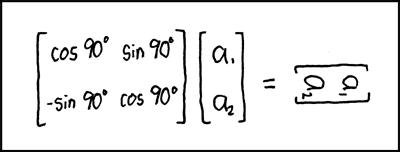
\includegraphics{xkcd.png} \\
    \footnotesize\sffamily%
    Tiré de \href{http://xkcd.com/184/}{XKCD.com}
  \end{minipage}
  \setkeys{Gin}{width=0.8\textwidth}
\end{vplace}
\cleardoublepage

\mainmatter

\include{notions_fondamentales}
\include{valeurs_propres}
\chapter{Décomposition LU}
\label{chap:decomposition}

%%%
%%% Fichers de solutions et de réponses
%%%

\Opensolutionfile{reponses}[reponses-decomposition_lu]
\Opensolutionfile{solutions}[solutions-decomposition_lu]

\begin{Filesave}{reponses}
\bigskip
\section*{Réponses}

\end{Filesave}

\begin{Filesave}{solutions}
\section*{Chapitre \ref{chap:decomposition}}
\addcontentsline{toc}{section}{Chapitre \protect\ref{chap:decomposition}}

\end{Filesave}

%%%
%%% Début des exercices
%%%

\begin{exercice}
  Résoudre le système d'équations
  \begin{displaymath}
    \begin{array}[t]{*{2}{r@{\;}c@{\;}}r@{\;=\;}r}
      3x_1 &-& 6x_2 &-& 3x_3 &  -3 \\
      2x_1 & &      &+& 6x_3 & -22 \\
      -4x_1&+& 7x_2 &+& 4x_3 &   3
    \end{array}
  \end{displaymath}
  par la décomposition $LU$ sachant que
  \begin{displaymath}
    \begin{bmatrix}
      3 & -6 & -3 \\ 2 & 0 & 6 \\ -4 & 7 & 4
    \end{bmatrix} =
    \begin{bmatrix}
      3 & 0 & 0 \\ 2 & 4 & 0 \\ -4 & -1 & 2
    \end{bmatrix}
    \begin{bmatrix}
      1 & -2 & -1 \\ 0 & 1 & 2 \\ 0 & 0 & 1
    \end{bmatrix}.
  \end{displaymath}
  \begin{sol}
    La matrice
    \begin{displaymath}
      \mat{A} =
      \begin{bmatrix}
        3 & -6 & -3 \\ 2 & 0 & 6 \\ -4 & 7 & 4
      \end{bmatrix}
    \end{displaymath}
    est exprimée sous la forme $\mat{A} = \mat{L} \mat{U}$, où
    \begin{align*}
      \mat{L}
      &=
      \begin{bmatrix}
        3 & 0 & 0 \\ 2 & 4 & 0 \\ -4 & -1 & 2
      \end{bmatrix} \\
      \intertext{et}
      \mat{U}
      &=
      \begin{bmatrix}
        1 & -2 & -1 \\ 0 & 1 & 2 \\ 0 & 0 & 1
      \end{bmatrix}.
    \end{align*}
    Ainsi, le système d'équations $\mat{A} \mat{x} = \mat{b}$ (où
    $\mat{b} = (-3, -22, 3)^T$) peut être exprimé sous la forme
    $\mat{L} \mat{U} \mat{x} = \mat{b}$, soit $\mat{L} \mat{y} =
    \mat{b}$ et $\mat{U} \mat{x} = \mat{y}$. On résoud tout d'abord
    $\mat{L} \mat{y} = \mat{b}$ par simple substitution successive. On
    trouve
    \begin{align*}
      y_1 &= - 1 \\
      y_2 &= \frac{-22 - 2 y_1}{4} = -5 \\
      y_3 &= \frac{3 + 4 y_1 + y_2}{2} = -3.
    \end{align*}
    Par la suite, on résoud de même $\mat{U} \mat{x} = \mat{y}$, ce
    qui donne
    \begin{align*}
      x_3 &= -3 \\
      x_2 &= -5 - 2 x_3 = 1 \\
      x_1 &= -1 + 2 x_2 + x_3 = -2.
    \end{align*}
  \end{sol}
  \begin{rep}
    $x_1 = -2$, $x_2 = 1$, $x_3 = -3$
  \end{rep}
\end{exercice}

\begin{exercice}
  Soit
  \begin{align*}
    \mat{E}_1
    &= \begin{bmatrix} 1&0 \\ 2&3 \end{bmatrix} \\
    \mat{E}_2
    &= \begin{bmatrix} \frac{1}{3}&0 \\ 0&\frac{1}{3} \end{bmatrix} \\
    \intertext{et}
    \mat{A}
    &= \mat{E}_1^{-1} \mat{E}_2^{-1}
    \begin{bmatrix} 1&-2 \\ 0&1 \end{bmatrix}.
  \end{align*}
  Résoudre le système d'équations
  \begin{displaymath}
    \mat{A} \mat{x} = \begin{bmatrix} 0\\1 \end{bmatrix}
  \end{displaymath}
  par la décomposition $LU$.
  \begin{sol}
    On cherche tout d'abord des matrices triangulaires inférieure et
    supérieure $\mat{L}$ et $\mat{U}$, respectivement, tel que
    $\mat{A} = \mat{L} \mat{U}$. On nous donne dans l'énoncé
    \begin{displaymath}
      \mat{A} = \mat{E}_1^{-1} \mat{E}_2^{-1}
      \begin{bmatrix} 1&-2 \\ 0&1 \end{bmatrix},
    \end{displaymath}
    d'où
    \begin{displaymath}
      \mat{U} = \begin{bmatrix} 1&-2 \\ 0&1 \end{bmatrix},
    \end{displaymath}
    et $\mat{L} = \mat{E}_1^{-1} \mat{E}_2^{-1}$. Or,
    \begin{align*}
      \mat{E}_1^{-1}
      &= \frac{1}{3} \begin{bmatrix} 3&0 \\ -2&1 \end{bmatrix} \\
      \mat{E}_2^{-1}
      &= \begin{bmatrix} 3&0 \\ 0&3 \end{bmatrix} \\
      &= 3 \mat{I}
      \intertext{et, par conséquent,}
      \mat{L}
      &= \begin{bmatrix} 3&0 \\ -2&1 \end{bmatrix}.
    \end{align*}
    Pour résoudre par décomposition $LU$ le système d'équations
    $\mat{A} \mat{x} = \mat{L} \mat{U} \mat{x} = \mat{b}$, où $\mat{b}
    = (0, 1)$, on pose $\mat{U} \mat{x} = \mat{y}$ et résout d'abord
    $\mat{L} \mat{y} = \mat{b}$ par substitution. On a donc le système
    d'équations
    \begin{displaymath}
      \begin{bmatrix} 3&0 \\ -2&1 \end{bmatrix}
      \begin{bmatrix} y_1 \\ y_2 \end{bmatrix} =
      \begin{bmatrix} 0\\1 \end{bmatrix},
    \end{displaymath}
    dont la solution est $y_1 = 0$ et $y_2 = 1$. Par la suite, on a
    \begin{displaymath}
      \begin{bmatrix} 1&-2 \\ 0&1 \end{bmatrix}
      \begin{bmatrix} x_1 \\ x_2 \end{bmatrix} =
      \begin{bmatrix} 0\\1 \end{bmatrix},
    \end{displaymath}
    d'où, finalement, $x_1 = 1$ et $x_2 = 2$.
  \end{sol}
  \begin{rep}
    $\mat{x} = (1, 2)$
  \end{rep}
\end{exercice}

\Closesolutionfile{reponses}
\Closesolutionfile{solutions}

%%%
%%% Insérer les réponses
%%%
\input{reponses-decomposition_lu}


%%% Local Variables:
%%% mode: latex
%%% TeX-master: exercices_methodes_numeriques
%%% End:


\appendix
%%% Copyright (C) 2018 Vincent Goulet
%%%
%%% Ce fichier fait partie du projet
%%% «Méthodes numériques en actuariat avec R»
%%% http://github.com/vigou3/methodes-numeriques-en-actuariat
%%%
%%% Cette création est mise à disposition selon le contrat
%%% Attribution-Partage dans les mêmes conditions 4.0
%%% International de Creative Commons.
%%% http://creativecommons.org/licenses/by-sa/4.0/

\chapter{Solutions des exercices}
\label{chap:solutions}
\markboth{Solutions des exercices}{Solutions des exercices}

\begingroup

%% Environnement Schunk simplifié pour l'affichage des réponses
\renewenvironment{Schunk}{%
  \setlength{\topsep}{0pt}
  \colorlet{shadecolor}{codebg}
  \begin{snugshade*}}%
  {\end{snugshade*}}
\input{solutions-generation}
\input{solutions-simulation}
\input{solutions-montecarlo}

\endgroup

%%% Local Variables:
%%% mode: latex
%%% TeX-engine: xetex
%%% TeX-master: "methodes-numeriques-en-actuariat_simulation"
%%% coding: utf-8
%%% End:


\bibliography{r,math,stat,informatique,vg}

\cleartoverso
\thispagestyle{empty}
\vspace*{\fill}

\begingroup
\calccentering{\unitlength}
\begin{adjustwidth*}{\unitlength}{-\unitlength}
  \begin{flushleft}
    \small %
    Ce document a été produit avec le système de mise en page
    {\XeLaTeX}. Le texte principal est en Lucida Bright~OT 11~points,
    les mathématiques en Lucida Bright Math~OT, le code informatique
    en Lucida Grande Mono~DK et les titres en Adobe Myriad~Pro. Des
    icônes proviennent de la police Font~Awesome. Les graphiques ont
    été réalisés avec R.
  \end{flushleft}
\end{adjustwidth*}
\endgroup
\vfill


\cleartoverso
%%% Copyright (C) 2018 Vincent Goulet
%%%
%%% Ce fichier fait partie du projet
%%% «Méthodes numériques en actuariat avec R»
%%% http://github.com/vigou3/methodes-numeriques-en-actuariat
%%%
%%% Cette création est mise à disposition selon le contrat
%%% Attribution-Partage dans les mêmes conditions 4.0
%%% International de Creative Commons.
%%% http://creativecommons.org/licenses/by-sa/4.0/

\begingroup

\TPGrid{3}{36}
\textblockorigin{0mm}{0mm}
\setlength{\parindent}{0mm}
\setlength{\banderougewidth}{2\TPHorizModule}
\setlength{\bandeorwidth}{\TPHorizModule}
\setlength{\gapwidth}{2pt}
\addtolength{\bandeorwidth}{-\gapwidth}

%% bandeau identitaire arrière
\begin{textblock*}{8.5in}[0,1](0mm,30\TPVertModule)
  \textcolor{or}{\rule{\bandeorwidth}{\TPVertModule}}%      % bande or
  \rule{\gapwidth}{0pt}%                                    % filet
  \textcolor{rouge}{\rule{\banderougewidth}{\TPVertModule}} % bande rouge
\end{textblock*}

% code-barre
% \begin{textblock*}{0.9\TPHorizModule}(0.1\TPHorizModule,25\TPVertModule)
%   \includegraphics[height=4\TPVertModule]{codebarre_\ISBN}
% \end{textblock*}

\endgroup


\end{document}

%%% Local Variables:
%%% mode: latex
%%% TeX-engine: xetex
%%% TeX-master: t
%%% coding: utf-8
%%% End:
